In the conventional approach to distributed databases, the CPU orchestrates data transfer between nodes. When using this CPU-initiated communication model, the CPU copies data from the GPU device memory to main memory.

GPUDirect \cite{gilad2011} makes it possible to avoid this copy overhead by sending data directly from the GPU.
This improved communication model using GPUDirect has a significant impact on performance, but the latency introduced from CPU initiation still leaves room for improvement: namely the removal of the CPU entirely from the communication pipeline.
This is possible with the NVSHMEM library from NVIDIA using strategies discussed in this section.

The following figures illustrate the difference in critical sections between the two approaches.

\begin{figure}[h]
    \centering
    \captionsetup{justification=centering}
    \path (0,300); %set diagram left start at 0, and has height of 300

    %Rounded Rect [id:dp602011306068072] 
    \draw   (21,106.8) .. controls (21,91.45) and (33.45,79) .. (48.8,79) -- (236.2,79) .. controls (251.55,79) and (264,91.45) .. (264,106.8) -- (264,190.2)     .. controls (264,205.55) and (251.55,218) .. (236.2,218) -- (48.8,218) .. controls (33.45,218) and (21,205.55) .. (21,190.2) -- cycle ;
    %Rounded Rect [id:dp18758960033065608] 
    \draw   (396,107.8) .. controls (396,92.45) and (408.45,80) .. (423.8,80) -- (611.2,80) .. controls (626.55,80) and (639,92.45) .. (639,107.8) --     (639,191.2) .. controls (639,206.55) and (626.55,219) .. (611.2,219) -- (423.8,219) .. controls (408.45,219) and (396,206.55) .. (396,191.2) -- cycle ;
    %Rounded Rect [id:dp6120664204960634] 
    \draw   (40,104.95) .. controls (40,97.25) and (46.25,91) .. (53.95,91) -- (95.8,91) .. controls (103.5,91) and (109.75,97.25) .. (109.75,104.95) --     (109.75,186.3) .. controls (109.75,194) and (103.5,200.25) .. (95.8,200.25) -- (53.95,200.25) .. controls (46.25,200.25) and (40,194) .. (40,186.3) --     cycle [fill={rgb:green,1;yellow,1;pink,0}];
    %Rounded Rect [id:dp21812393541423936] 
    \draw   (551,103.95) .. controls (551,96.25) and (557.25,90) .. (564.95,90) -- (606.8,90) .. controls (614.5,90) and (620.75,96.25) .. (620.75,103.95) --     (620.75,185.3) .. controls (620.75,193) and (614.5,199.25) .. (606.8,199.25) -- (564.95,199.25) .. controls (557.25,199.25) and (551,193) .. (551,185.3)     -- cycle [fill={rgb:green,1;yellow,1;pink,0}] ;
    %Rounded Rect [id:dp5570992455242908] 
    \draw   (131,101.05) .. controls (131,95.64) and (135.39,91.25) .. (140.8,91.25) -- (238.95,91.25) .. controls (244.36,91.25) and (248.75,95.64) ..     (248.75,101.05) -- (248.75,130.45) .. controls (248.75,135.86) and (244.36,140.25) .. (238.95,140.25) -- (140.8,140.25) .. controls (135.39,140.25) and     (131,135.86) .. (131,130.45) -- cycle ;
    %Rounded Rect [id:dp9865384483688472] 
    \draw   (412,101.05) .. controls (412,95.64) and (416.39,91.25) .. (421.8,91.25) -- (519.95,91.25) .. controls (525.36,91.25) and (529.75,95.64) ..     (529.75,101.05) -- (529.75,130.45) .. controls (529.75,135.86) and (525.36,140.25) .. (519.95,140.25) -- (421.8,140.25) .. controls (416.39,140.25) and     (412,135.86) .. (412,130.45) -- cycle;
    %Shape: Rectangle [id:dp5183376461620953] 
    \draw   (130,150) -- (250.75,150) -- (250.75,199.25) -- (130,199.25) -- cycle ;
    %Shape: Rectangle [id:dp2368467260325865] 
    \draw   (410,151) -- (530.75,151) -- (530.75,200.25) -- (410,200.25) -- cycle ;
    %Left Right Arrow [id:dp5286461875079793] 
    \draw  [fill={rgb, 255:red, 204; green, 76; blue, 3 }  ,fill opacity=1 ] (85.3,114.25) -- (102.8,104.25) -- (102.8,109.25) -- (137.8,109.25) --     (137.8,104.25) -- (155.3,114.25) -- (137.8,124.25) -- (137.8,119.25) -- (102.8,119.25) -- (102.8,124.25) -- cycle ;
    %Left Right Arrow [id:dp2994575111375585] 
    \draw  [fill={rgb, 255:red, 204; green, 76; blue, 3 }  ,fill opacity=1 ] (505.3,110.25) -- (522.8,100.25) -- (522.8,105.25) -- (557.8,105.25) --     (557.8,100.25) -- (575.3,110.25) -- (557.8,120.25) -- (557.8,115.25) -- (522.8,115.25) -- (522.8,120.25) -- cycle ;
    %Left Right Arrow [id:dp9904840465412947] 
    \draw  [fill={rgb, 255:red, 204; green, 76; blue, 3 }  ,fill opacity=1 ] (243.75,174.35) -- (267.57,165.25) -- (267.57,171.53) -- (392.93,171.53) --     (392.93,165.25) -- (416.75,174.35) -- (392.93,183.45) -- (392.93,177.17) -- (267.57,177.17) -- (267.57,183.45) -- cycle ;
    %Left Right Arrow [id:dp47754037113398307] 
    \draw  [fill={rgb, 255:red, 204; green, 76; blue, 3 }  ,fill opacity=1 ] (86.3,177.25) -- (103.8,167.25) -- (103.8,172.25) -- (138.8,172.25) --     (138.8,167.25) -- (156.3,177.25) -- (138.8,187.25) -- (138.8,182.25) -- (103.8,182.25) -- (103.8,187.25) -- cycle ;
    %Left Right Arrow [id:dp7512448088396187] 
    \draw  [fill={rgb, 255:red, 204; green, 76; blue, 3 }  ,fill opacity=1 ] (505.3,177.25) -- (522.8,167.25) -- (522.8,172.25) -- (557.8,172.25) --     (557.8,167.25) -- (575.3,177.25) -- (557.8,187.25) -- (557.8,182.25) -- (522.8,182.25) -- (522.8,187.25) -- cycle ;

    \draw (74.88,145.63) node   [align=left] {CPU};
    \draw (585.88,144.63) node   [align=left] {CPU};
    \draw (182.25,115.5) node   [align=left] {GPU};
    \draw (470.88,115.75) node   [align=left] {GPU};
    \draw (186.92,174.5) node   [align=left] {NIC};
    \draw (470.38,175.63) node   [align=left] {NIC};
    \caption{Communication with CPU in critical path}
    \label{fig:cpu_in_crit}
\end{figure}

In Figure \ref{fig:cpu_in_crit}, the CPU is included in the critical communication path, incurring a latency penalty.
The following Figure \ref{fig:cpu_out_crit} shows the critical communication path in the GPU initiated approach, which no longer includes the CPU.

\begin{figure}[h]
    \centering
    \captionsetup{justification=centering}
    \path (0,300); %set diagram left start at 0, and has height of 300

    %Rounded Rect [id:dp602011306068072] 
    \draw   (21,106.8) .. controls (21,91.45) and (33.45,79) .. (48.8,79) -- (236.2,79) .. controls (251.55,79) and (264,91.45) .. (264,106.8) -- (264,190.2)     .. controls (264,205.55) and (251.55,218) .. (236.2,218) -- (48.8,218) .. controls (33.45,218) and (21,205.55) .. (21,190.2) -- cycle ;
    %Rounded Rect [id:dp18758960033065608] 
    \draw   (396,107.8) .. controls (396,92.45) and (408.45,80) .. (423.8,80) -- (611.2,80) .. controls (626.55,80) and (639,92.45) .. (639,107.8) --     (639,191.2) .. controls (639,206.55) and (626.55,219) .. (611.2,219) -- (423.8,219) .. controls (408.45,219) and (396,206.55) .. (396,191.2) -- cycle ;
    %Rounded Rect [id:dp6120664204960634] 
    \draw   (40,104.95) .. controls (40,97.25) and (46.25,91) .. (53.95,91) -- (95.8,91) .. controls (103.5,91) and (109.75,97.25) .. (109.75,104.95) --     (109.75,186.3) .. controls (109.75,194) and (103.5,200.25) .. (95.8,200.25) -- (53.95,200.25) .. controls (46.25,200.25) and (40,194) .. (40,186.3) --     cycle [fill=black!40]; 
    %Rounded Rect [id:dp21812393541423936] 
    \draw   (551,103.95) .. controls (551,96.25) and (557.25,90) .. (564.95,90) -- (606.8,90) .. controls (614.5,90) and (620.75,96.25) .. (620.75,103.95) --     (620.75,185.3) .. controls (620.75,193) and (614.5,199.25) .. (606.8,199.25) -- (564.95,199.25) .. controls (557.25,199.25) and (551,193) .. (551,185.3)     -- cycle [fill=black!40];
    %Rounded Rect [id:dp5570992455242908] 
    \draw   (131,101.05) .. controls (131,95.64) and (135.39,91.25) .. (140.8,91.25) -- (238.95,91.25) .. controls (244.36,91.25) and (248.75,95.64) ..     (248.75,101.05) -- (248.75,130.45) .. controls (248.75,135.86) and (244.36,140.25) .. (238.95,140.25) -- (140.8,140.25) .. controls (135.39,140.25) and     (131,135.86) .. (131,130.45) -- cycle ;
    %Rounded Rect [id:dp9865384483688472] 
    \draw   (412,101.05) .. controls (412,95.64) and (416.39,91.25) .. (421.8,91.25) -- (519.95,91.25) .. controls (525.36,91.25) and (529.75,95.64) ..     (529.75,101.05) -- (529.75,130.45) .. controls (529.75,135.86) and (525.36,140.25) .. (519.95,140.25) -- (421.8,140.25) .. controls (416.39,140.25) and     (412,135.86) .. (412,130.45) -- cycle ;
    %Shape: Rectangle [id:dp5183376461620953] 
    \draw   (130,150) -- (250.75,150) -- (250.75,199.25) -- (130,199.25) -- cycle ;
    %Shape: Rectangle [id:dp2368467260325865] 
    \draw   (410,151) -- (530.75,151) -- (530.75,200.25) -- (410,200.25) -- cycle ;
    %Left Right Arrow [id:dp9904840465412947] 
    \draw  [fill={rgb, 255:red, 204; green, 76; blue, 3 }  ,fill opacity=1 ] (243.75,174.35) -- (267.57,165.25) -- (267.57,171.53) -- (392.93,171.53) --     (392.93,165.25) -- (416.75,174.35) -- (392.93,183.45) -- (392.93,177.17) -- (267.57,177.17) -- (267.57,183.45) -- cycle ;
    %Left Right Arrow [id:dp47754037113398307] 
    \draw  [fill={rgb, 255:red, 204; green, 76; blue, 3 }  ,fill opacity=1 ] (191.03,129.25) -- (202.75,137.25) -- (196.89,137.25) -- (196.89,153.25) --     (202.75,153.25) -- (191.03,161.25) -- (179.3,153.25) -- (185.16,153.25) -- (185.16,137.25) -- (179.3,137.25) -- cycle ;
    %Left Right Arrow [id:dp2871368640426972] 
    \draw  [fill={rgb, 255:red, 204; green, 76; blue, 3 }  ,fill opacity=1 ] (472.03,129.25) -- (483.75,137.25) -- (477.89,137.25) -- (477.89,153.25) --     (483.75,153.25) -- (472.03,161.25) -- (460.3,153.25) -- (466.16,153.25) -- (466.16,137.25) -- (460.3,137.25) -- cycle ;
    
    % Text Node
    \draw (74.88,145.63) node   [align=left] {CPU};
    % Text Node
    \draw (585.88,144.63) node   [align=left] {CPU};
    % Text Node
    \draw (182.25,115.5) node   [align=left] {GPU};
    % Text Node
    \draw (470.88,115.75) node   [align=left] {GPU};
    % Text Node
    \draw (186.92,174.5) node   [align=left] {NIC};
    % Text Node
    \draw (470.38,175.63) node   [align=left] {NIC};
    
    
    \caption{Communication with CPU out of critical path}
    \label{fig:cpu_out_crit}
\end{figure}

This paper explores this idea and its challenges using the NVSHMEM library for GPU-to-GPU communication, bypassing the latency introduced by the CPU.
Specifically, it analyzes the performance characteristics of NVSHMEM, and whether it provides a significant benefit for database workloads.

While the latency may be significantly improved with this approach, it is possible that additional complexity or issues in other metrics such as throughput make this approach unrealistic.

\clearpage

\subsection{Kernel Launch Overhead}

A common GPU programming model involves launching compute-heavy kernels on the device (GPU) and returning control to the host (CPU) before the next kernel launch.
The following Figure \ref{fig:kernel_launch_overhead} quantifies the impact of these kernel launches to assess whether this is an area of potential optimization.

\begin{figure}[h]
    \centering
    \captionsetup{justification=centering}
    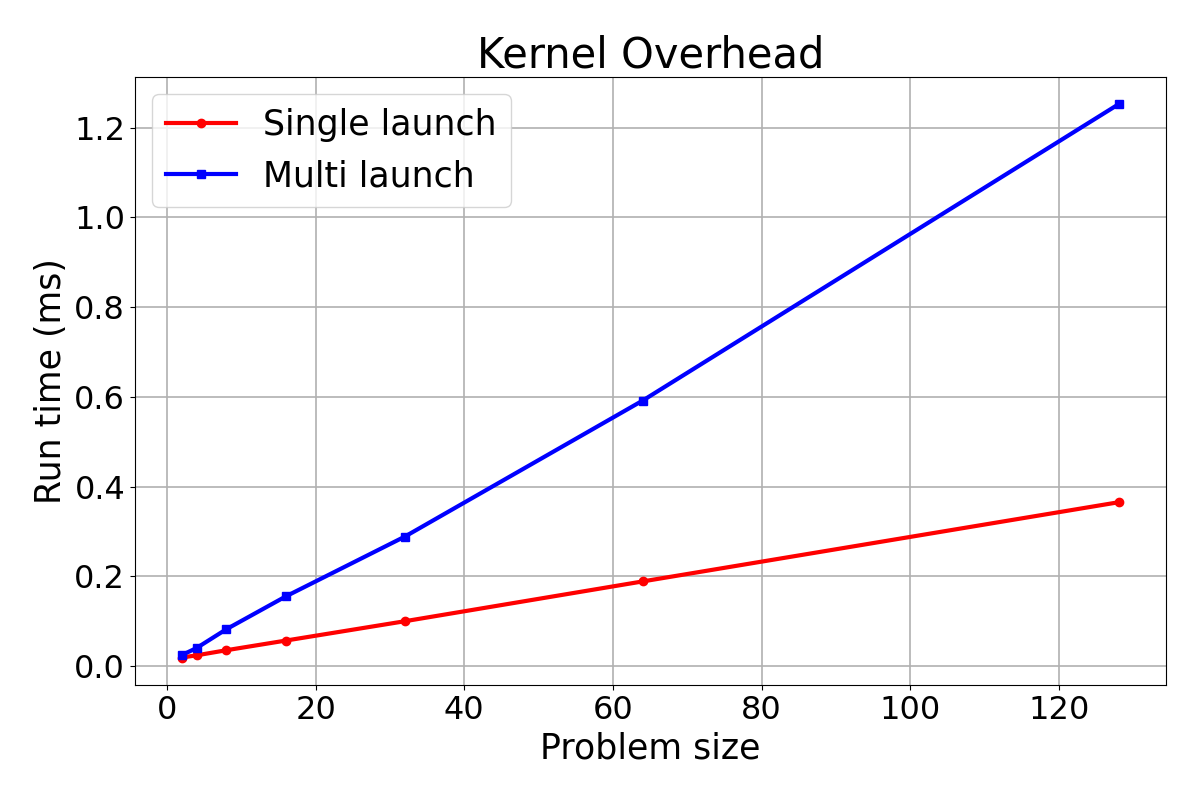
\includegraphics[width=0.4\textwidth]{img/overhead.png}
    \caption{Kernel launch overhead}
    \label{fig:kernel_launch_overhead}
\end{figure}

In this experiment, a progressively increasing problem size is tested with different kernel granularities.
The \enquote{Single launch} configuration uses a larger kernel, which is only be launched once.
On the other hand, the \enquote{Multi launch} configuration splits the work instead into smaller kernels which are launched separately.
Even though the same amount of work is completed by each configuration for a given problem size, there is a measurable increase in the kernel overhead - the time it takes to launch a kernel - for multiple kernel launches.

This serves as an important motivation to reduce the number of kernel launches in latency sensitive applications such as databases.
The problem with reducing the number of kernel launches in traditional CPU-initiated communication is that the CPU's control of the communication requires kernels to be much more fine-grained.

However, with the NVSHMEM programming model, it is possible to have much longer running kernels working more independently from the CPU, which would significantly reduce overhead induced from kernel launches.

\subsection{Programming Model}

NVSHMEM employs a programming model inspired by HPC-style computing, with the focus on cluster-wide symmetric memory exchanges.
The following Figure \ref{fig:nvshmem_sym_mem} illustrates the idea behind this symmetric memory model.

\begin{figure}[h]
    \centering
    \captionsetup{justification=centering}
    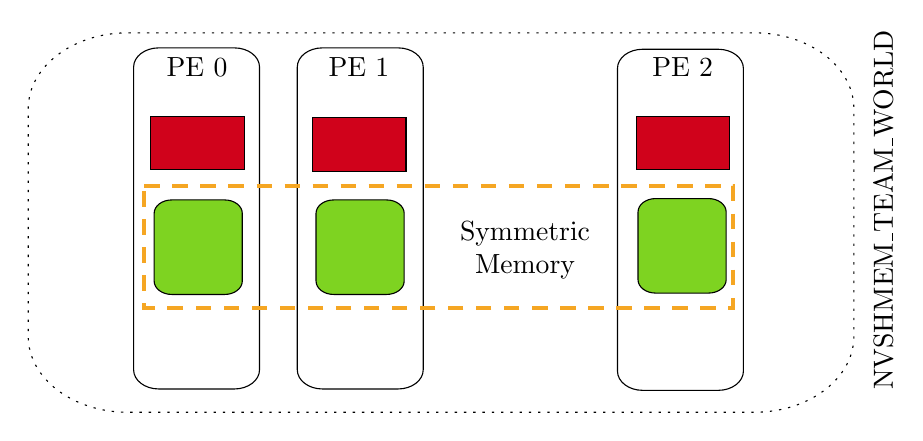
\begin{tikzpicture}[x=1pt,y=0.9pt,yscale=-0.55,xscale=0.65]
    %Rounded Rect [id:dp5682014849782169] 
    \draw   (100,34.25) .. controls (100,26.52) and (106.27,20.25) .. (114,20.25) -- (156,20.25) .. controls (163.73,20.25) and (170,26.52) .. (170,34.25) -- (170,255.25) .. controls (170,262.98) and (163.73,269.25) .. (156,269.25) -- (114,269.25) .. controls (106.27,269.25) and (100,262.98) .. (100,255.25) -- cycle ;
    %Rounded Rect [id:dp5262477048147362] 
    \draw   (191,34.25) .. controls (191,26.52) and (197.27,20.25) .. (205,20.25) -- (247,20.25) .. controls (254.73,20.25) and (261,26.52) .. (261,34.25) -- (261,255.25) .. controls (261,262.98) and (254.73,269.25) .. (247,269.25) -- (205,269.25) .. controls (197.27,269.25) and (191,262.98) .. (191,255.25) -- cycle ;
    %Rounded Rect [id:dp7573581856079369] 
    \draw   (369,35.25) .. controls (369,27.52) and (375.27,21.25) .. (383,21.25) -- (425,21.25) .. controls (432.73,21.25) and (439,27.52) .. (439,35.25) -- (439,256.25) .. controls (439,263.98) and (432.73,270.25) .. (425,270.25) -- (383,270.25) .. controls (375.27,270.25) and (369,263.98) .. (369,256.25) -- cycle ;
    %Shape: Rectangle [id:dp7570532028079713] 
    \draw  [fill={rgb, 255:red, 208; green, 2; blue, 27 }  ,fill opacity=1 ] (109.42,70.25) -- (161.42,70.25) -- (161.42,109.25) -- (109.42,109.25) -- cycle ;
    %Shape: Rectangle [id:dp19421520470566733] 
    \draw  [fill={rgb, 255:red, 208; green, 2; blue, 27 }  ,fill opacity=1 ] (199.42,71.25) -- (251.42,71.25) -- (251.42,110.25) -- (199.42,110.25) -- cycle ;
    %Shape: Rectangle [id:dp32300543498141965] 
    \draw  [fill={rgb, 255:red, 208; green, 2; blue, 27 }  ,fill opacity=1 ] (379.42,70.25) -- (431.42,70.25) -- (431.42,109.25) -- (379.42,109.25) -- cycle ;
    %Rounded Rect [id:dp6580910781722736] 
    \draw  [fill={rgb, 255:red, 126; green, 211; blue, 33 }  ,fill opacity=1 ] (111.42,141.05) .. controls (111.42,135.64) and (115.8,131.25) .. (121.22,131.25) -- (150.62,131.25) .. controls (156.03,131.25) and (160.42,135.64) .. (160.42,141.05) -- (160.42,190.45) .. controls (160.42,195.86) and (156.03,200.25) .. (150.62,200.25) -- (121.22,200.25) .. controls (115.8,200.25) and (111.42,195.86) .. (111.42,190.45) -- cycle ;
    %Rounded Rect [id:dp26363692092381197] 
    \draw  [fill={rgb, 255:red, 126; green, 211; blue, 33 }  ,fill opacity=1 ] (201.42,141.05) .. controls (201.42,135.64) and (205.8,131.25) .. (211.22,131.25) -- (240.62,131.25) .. controls (246.03,131.25) and (250.42,135.64) .. (250.42,141.05) -- (250.42,190.45) .. controls (250.42,195.86) and (246.03,200.25) .. (240.62,200.25) -- (211.22,200.25) .. controls (205.8,200.25) and (201.42,195.86) .. (201.42,190.45) -- cycle ;
    %Rounded Rect [id:dp18887280028716125] 
    \draw  [fill={rgb, 255:red, 126; green, 211; blue, 33 }  ,fill opacity=1 ] (380.42,140.05) .. controls (380.42,134.64) and (384.8,130.25) .. (390.22,130.25) -- (419.62,130.25) .. controls (425.03,130.25) and (429.42,134.64) .. (429.42,140.05) -- (429.42,189.45) .. controls (429.42,194.86) and (425.03,199.25) .. (419.62,199.25) -- (390.22,199.25) .. controls (384.8,199.25) and (380.42,194.86) .. (380.42,189.45) -- cycle ;
    %Rounded Rect [id:dp5265848887584798] 
    \draw  [color={rgb, 255:red, 0; green, 0; blue, 0 }  ,draw opacity=1 ][dash pattern={on 0.84pt off 2.51pt}] (41.42,64.65) .. controls (41.42,34.05) and (66.22,9.25) .. (96.82,9.25) -- (445.02,9.25) .. controls (475.61,9.25) and (500.42,34.05) .. (500.42,64.65) -- (500.42,230.85) .. controls (500.42,261.45) and (475.61,286.25) .. (445.02,286.25) -- (96.82,286.25) .. controls (66.22,286.25) and (41.42,261.45) .. (41.42,230.85) -- cycle ;
    %Shape: Rectangle [id:dp9039242900086101] 
    \draw  [color={rgb, 255:red, 245; green, 166; blue, 35 }  ,draw opacity=1 ][dash pattern={on 5.63pt off 4.5pt}][line width=1.5]  (106,121) -- (433.42,121) -- (433.42,210.25) -- (106,210.25) -- cycle ;
    
    % Text Node
    \draw (135.26,34.5) node   [align=left] {PE 0};
    % Text Node
    \draw (225.26,34.5) node   [align=left] {PE 1};
    % Text Node
    \draw (405.26,34.5) node   [align=left] {PE 2};
    % Text Node
    \draw (510,272) node [anchor=north west][inner sep=0.8pt]  [rotate=-270] [align=left] {NVSHMEM\_TEAM\_WORLD};
    % Text Node
    \draw (280,145) node [anchor=north west][inner sep=0.75pt]   [align=center] {Symmetric \\ Memory};
\end{tikzpicture}

    \caption{NVSHMEM symmetric memory model}
    \label{fig:nvshmem_sym_mem}
\end{figure}

In this model, a PE (Processing Element) represents a group of operating system processes, which may be executed on one or more nodes in a GPU cluster\cite{NVSHMEM2023}.
However, while it is possible to launch multiple PEs on a single GPU, this is not a recommended configuration in a production deployment, so this paper will focus on configurations with one PE per GPU and one GPU per node.

In this paper, we use NVSHMEM primitives for collective communication such as \textit{fcollect} to exchange local portions of a symmetrically allocated block with all the other PEs in the cluster.
Additionally, calls such as \textit{put\_nbi} are used for direct PE-to-PE communication.

Leveraging NVSHMEM allows us to reduce CPU involvement in data exchanges for benefits such as reduced communication latency.
However, this comes at the cost of a more complex programming model.
Compared to traditional distributed database approaches, using NVSHMEM for CPU independent communication is significantly more complex.

% - explain the difference between CPU- and GPU-initiated communicatoin
% - Explain the potential advantage of GPU-initiated communication: less kernel launch overhead, less CPU utilization, easier balance between compute and networking w/ async calls